\documentclass[12pt]{beamer}
\usepackage{../Estilos/BeamerFC}
\usepackage{../Estilos/ColoresLatex}
\usepackage{courier}
\usepackage{listingsutf8}
\usepackage{listings}
\usepackage{xcolor}
\usepackage{textcomp}
\usepackage{color}
\definecolor{deepblue}{rgb}{0,0,0.5}
\definecolor{brown}{rgb}{0.59, 0.29, 0.0}
\definecolor{OliveGreen}{rgb}{0,0.25,0}
% \usepackage{minted}

\DeclareCaptionFont{white}{\color{white}}
\DeclareCaptionFormat{listing}{\colorbox{gray}{\parbox{0.98\textwidth}{#1#2#3}}}
\captionsetup[lstlisting]{format=listing,labelfont=white,textfont=white}
\renewcommand{\lstlistingname}{Código}


\definecolor{Code}{rgb}{0,0,0}
\definecolor{Keywords}{rgb}{255,0,0}
\definecolor{Strings}{rgb}{255,0,255}
\definecolor{Comments}{rgb}{0,0,255}
\definecolor{Numbers}{rgb}{255,128,0}

\makeatletter

\newif\iffirstchar\firstchartrue
\newif\ifstartedbyadigit
\newif\ifprecededbyequalsign

\newcommand\processletter
{%
  \ifnum\lst@mode=\lst@Pmode%
    \iffirstchar%
        \global\startedbyadigitfalse%
      \fi
      \global\firstcharfalse%
    \fi
}

\newcommand\processdigit
{%
  \ifnum\lst@mode=\lst@Pmode%
      \iffirstchar%
        \global\startedbyadigittrue%
      \fi
      \global\firstcharfalse%
  \fi
}

\lst@AddToHook{OutputOther}%
{%
  \lst@IfLastOtherOneOf{=}
    {\global\precededbyequalsigntrue}
    {}%
}

\lst@AddToHook{Output}%
{%
  \ifprecededbyequalsign%
      \ifstartedbyadigit%
        \def\lst@thestyle{\color{orange}}%
      \fi
    \fi
  \global\firstchartrue%
  \global\startedbyadigitfalse%
  \global\precededbyequalsignfalse%
}

\lstset{ 
language=Python,                % choose the language of the code
basicstyle=\footnotesize\ttfamily,       % the size of the fonts that are used for the code
numbers=left,                   % where to put the line-numbers
numberstyle=\scriptsize,      % the size of the fonts that are used for the line-numbers
stepnumber=1,                   % the step between two line-numbers. If it is 1 each line will be numbered
numbersep=5pt,                  % how far the line-numbers are from the code
backgroundcolor=\color{white},  % choose the background color. You must add \usepackage{color}
showspaces=false,               % show spaces adding particular underscores
showstringspaces=false,         % underline spaces within strings
showtabs=false,                 % show tabs within strings adding particular underscores
frame=single,   		% adds a frame around the code
tabsize=2,  		% sets default tabsize to 2 spaces
captionpos=t,   		% sets the caption-position to bottom
breaklines=true,    	% sets automatic line breaking
breakatwhitespace=false,    % sets if automatic breaks should only happen at whitespace
escapeinside={| |},  % if you want to add a comment within your code
stringstyle =\color{OliveGreen},
otherkeywords={as, np.array, np.concatenate, np.linspace, linspace, interpolate.interp1d, kind, plt.plot, .copy, np.arange, np.cos, np.pi, lw, ls, label, splrep, splev, plt.legend, loc, plt.title, plt.ylim, plt.show, sign, math.ceil, math.log, np.sqrt, np.exp, np.zeros, plt.xlabel, plt.ylabel, plt.xlim, np.identity, random, np.dot, np.outer, np.diagonal },             % Add keywords here
keywordstyle = \color{blue},
commentstyle = \color{darkcerulean},
identifierstyle = \color{black},
literate=%
         {á}{{\'a}}1
         {é}{{\'e}}1
         {í}{{\'i}}1
         {ó}{{\'o}}1
         {ú}{{\'u}}1
%
%keywordstyle=\ttb\color{deepblue}
%fancyvrb = true,
}

\lstdefinestyle{FormattedNumber}{%
    literate={0}{{\textcolor{red}{0}}}{1}%
             {1}{{\textcolor{red}{1}}}{1}%
             {2}{{\textcolor{red}{2}}}{1}%
             {3}{{\textcolor{red}{3}}}{1}%
             {4}{{\textcolor{red}{4}}}{1}%
             {5}{{\textcolor{red}{5}}}{1}%
             {6}{{\textcolor{red}{6}}}{1}%
             {7}{{\textcolor{red}{7}}}{1}%
             {8}{{\textcolor{red}{8}}}{1}%
             {9}{{\textcolor{red}{9}}}{1}%
             {.0}{{\textcolor{red}{.0}}}{2}% Following is to ensure that only periods
             {.1}{{\textcolor{red}{.1}}}{2}% followed by a digit are changed.
             {.2}{{\textcolor{red}{.2}}}{2}%
             {.3}{{\textcolor{red}{.3}}}{2}%
             {.4}{{\textcolor{red}{.4}}}{2}%
             {.5}{{\textcolor{red}{.5}}}{2}%
             {.6}{{\textcolor{red}{.6}}}{2}%
             {.7}{{\textcolor{red}{.7}}}{2}%
             {.8}{{\textcolor{red}{.8}}}{2}%
             {.9}{{\textcolor{red}{.9}}}{2}%
             {\ }{{ }}{1}% handle the space
         ,%
          %mathescape=true
          escapeinside={__}
          }



\usetheme{Dresden}
\usecolortheme{seahorse}
%\useoutertheme{default}
\setbeamercovered{invisible}
% or whatever (possibly just delete it)
\setbeamertemplate{section in toc}[sections numbered]
\setbeamertemplate{subsection in toc}[subsections numbered]
\setbeamertemplate{subsection in toc}{\leavevmode\leftskip=3.2em\rlap{\hskip-2em\inserttocsectionnumber.\inserttocsubsectionnumber}\inserttocsubsection\par}
\setbeamercolor{section in toc}{fg=blue}
\setbeamercolor{subsection in toc}{fg=blue}
\setbeamercolor{frametitle}{fg=blue}
\setbeamertemplate{caption}[numbered]

\setbeamertemplate{footline}
\beamertemplatenavigationsymbolsempty
\setbeamertemplate{headline}{}

\makeatletter
\setbeamercolor{section in foot}{bg=gray!30, fg=black!90!orange}
\setbeamercolor{subsection in foot}{bg=blue!30!yellow, fg=red}
\setbeamertemplate{footline}
{
  \leavevmode%
  \hbox{%
  \begin{beamercolorbox}[wd=.333333\paperwidth,ht=2.25ex,dp=1ex,center]{section in foot}%
    \usebeamerfont{section in foot} \insertsection
  \end{beamercolorbox}}%
  \begin{beamercolorbox}[wd=.333333\paperwidth,ht=2.25ex,dp=1ex,center]{subsection in foot}%
    \usebeamerfont{subsection in foot}  \insertsubsection
  \end{beamercolorbox}%
  \begin{beamercolorbox}[wd=.333333\paperwidth,ht=2.25ex,dp=1ex,right]{date in head/foot}%
    \usebeamerfont{date in head/foot} \insertshortdate{} \hspace*{2em}
    \insertframenumber{} / \inserttotalframenumber \hspace*{2ex} 
  \end{beamercolorbox}}%
  \vskip0pt%
\makeatother 

\makeatletter
\patchcmd{\beamer@sectionintoc}{\vskip1.5em}{\vskip0.8em}{}{}
\makeatother

% \usefonttheme{serif}

\title{\large{Integración numérica}}
\subtitle{Tema 2 - Operaciones matemáticas básicas}
\author{M. en C. Gustavo Contreras Mayén}
\date{}

\newtheorem{miteorema}{Teorema}

\begin{document}
\maketitle

\section*{Contenido}
\frame{\tableofcontents[currentsection, hideallsubsections]}

\section{Extrapolación de Richardson}
\frame{\tableofcontents[currentsection, hideothersubsections]}
\subsection{Definición}

\begin{frame}
\frametitle{Extrapolación de Richardson}
La Extrapolación de Richardson es un método sencillo para aumentar la precisión de ciertos procedimientos numéricos, incluyendo las aproximaciones por diferencias finitas.
\end{frame}
\begin{frame}
\frametitle{Extrapolación de Richardson}
\setbeamercolor{item projected}{bg=aliceblue,fg=black}
\setbeamertemplate{enumerate items}{%
\usebeamercolor[bg]{item projected}%
\raisebox{1.5pt}{\colorbox{bg}{\color{fg}\footnotesize\insertenumlabel}}%
}
\begin{enumerate}[<+->]
\item Supongamos que tenemos la forma de calcular una cantidad $G$.
\item Por otra parte, si consideramos que el resultado depende de un parámetro $h$,
\item Hagamos la aproximación por $g (h)$
\item Tenemos que $G = g (h) + E (h)$, donde $E (h)$ representa el error.
\end{enumerate}
\end{frame}
\begin{frame}
\frametitle{Avance en la extrapolación}
La extrapolación de Richardson puede remover el error, siempre que tenga la forma $E (h) = c \, h^{p}$, donde $c$ y $p$ son constantes. \pause Iniciamos el cálculo para varios valores de $h$, digamos $h = h_{1}$, así:
\pause
\begin{align*}
G = g (h_{1}) + c \, h_{1}^{p}
\end{align*}
\pause
Repetimos el cálculo con $h = h_{2}$, por tanto:
\pause
\begin{align*}
G = g (h_{2}) + c \, h_{2}^{p}
\end{align*}
\end{frame}
\begin{frame}
\frametitle{Recuperando $G$}
Eliminando $c$ y resolviendo para $G$, tenemos:
\pause
\begin{align*}
G = \dfrac{(h_{1}/h_{2})^{p} g(h_{2}) - g(h_{1})}{(h_{1}/h_{2})^{p}-1}
\end{align*}
que es la fórmula de Extrapolación de Richardson. En la práctica se usa $h_{2} = h_{1}/2$, quedando:
\pause
\begin{align*}
G = \dfrac{2^{p} g(h_{1}/2) - g(h_{1})}{2^{p}-1}
\end{align*}
\end{frame}
\begin{frame}
\frametitle{Ejemplo de la extrapolación de Richardsonº}
Usemos el ejemplo de $\big[ \exp(-x) \big]^{\prime \prime}$ en $x = 1$, calculada mediante diferencias finitas, consideremos los valores de la tabla con ocho dígitos.
\\
\bigskip
\pause
Dado que la extrapolación contine errores por truncamiento, debemos limitarnos a los valores de $h$ que producen redondeo insignificante.
\end{frame}
\begin{frame}
%\frametitle{Cálculo de la aproximación de la derivada}
\begin{table}
\centering
\renewcommand{\arraystretch}{0.8}
\begin{tabular}{c c c }
h & derivada & error \\ \hline
$0.64$    & $0.38060910$ & $3.460279e-02$ \\ \hline
$0.32$    & $0.37102941$ & $8.562517e-03$ \\ \hline
$0.16$    & $0.36866492$ & $2.135158e-03$ \\ \hline
$0.08$    & $0.36807569$ & $5.334503e-04$ \\ \hline
$0.04$    & $0.36792849$ & $1.333436e-04$ \\ \hline
$0.02$    & $0.36789170$ & $3.333696e-05$ \\ \hline
$0.01$    & $0.36788251$ & $8.336546e-06$ \\ \hline
$0.005$   & $0.36788021$ & $2.086520e-06$ \\ \hline
$0.0025$  & $0.36787963$ & $5.240152e-07$ \\ \hline
$0.00125$ & $0.36787949$ & $1.333059e-07$ \\ \hline
\hline
\end{tabular}
\end{table}
\end{frame}
\begin{frame}
\frametitle{Alcance del error}
De la tabla anterior que calculamos, tenemos que:
\pause
\begin{align*}
g (0.64) = 0.38060910 \hspace{2cm} g (0.32) = 0.37102941
\end{align*}
\pause
El error de truncamiento en la aproximación central por diferencias finitas es:
\pause
\begin{align*}
E (h) = \order{h^{2}} = c_{1} \, h^{2} + c_{2} \, h^{4} + c_{3} \, h^{6} + \ldots
\end{align*}
\end{frame}
\begin{frame}
\frametitle{Cancelando el término dominante}
Por lo que podemos eliminar el primer término del error (dominante), si usamos $p = 2$ y $h_{1} = 0.64$, así:
\pause
\begin{eqnarray*}
\begin{aligned}
G &= \dfrac{2^{2} \, g(0.32) - g(0.64}{2^{2} - 1} = \pause \dfrac{4 \, (0.37102941) - 0.38060910}{3} \\
&= 0.36783618
\end{aligned}
\end{eqnarray*}
Que es una aproximación de $\big[ \exp(-x) \big]^{\prime \prime}$ con un error del orden $\order{h^{4}}$. \pause Que es el mejor valor obtenido en comparación de los obtenidos con precisión de ocho dígitos.
\end{frame}
\begin{frame}
\frametitle{Segundo ejercicio extrapolación de Richardson}
Teniendo en cuenta los puntos de datos uniformemente espaciados:
\pause
\begin{table}
\centering
\begin{tabular}{c | c | c | c | c | c }
$x$ & $0$ & $0.1$ & $0.2$ & $0.3$ & $0.4$ \\ \hline
$f (x)$ & $0.0000$ & $0.0819$ & $0.1341$ & $0.1646$ & $0.1797$
\end{tabular}
\end{table}
Calcula $\pderivada{f} (x)$ y $\sderivada{f} (x)$ en $x = 0$ y $x = 0.2$, usando la aproximación por diferencias finitas de orden $\order{h^{2}}$.
\end{frame}
\begin{frame}
\frametitle{Solución}
Usando la aproximación por diferencias finitas de orden $\order{h^{2}}$, de la lista de diferencias hacia adelante, tenemos:
\pause 
\begin{eqnarray*}
\begin{aligned}
\pderivada{f} (0) &= \dfrac{-3 \, f (0) + 4 \, f (0.1) - f \, (0.2)}{2 \, (0.1)} = \pause 0.9675 \\[1em] \pause
\sderivada{f} (0) &= \dfrac{2 \, f (0) - 5 \, f (0.1) + 4 \, f (0.2) - f (0.3)}{(0.1)^{2}} =\pause  -3.77
\end{aligned}
\end{eqnarray*}
\end{frame}
\begin{frame}
\frametitle{Diferencias centrales de $\order{h^{2}}$}
Si usamos ahora la aproximación por diferencias centrales:
\pause
\begin{eqnarray*}
\begin{aligned}
\pderivada{f} (0.2) &= \dfrac{-f (0.1) + f (0.3)}{2 \, (0.1)} = 0.4135 \\[0.5em] \pause
\sderivada{f} (0.2) &= \dfrac{f (0.1) - 2 \, f (0.2) + f \, (0.3)}{(0.1)^{2}} = -2.17
\end{aligned}
\end{eqnarray*}
\end{frame}
\begin{frame}
\frametitle{Calculando el mejor valor posible}
Usando los siguientes datos del ejemplo anterior: calcula $\pderivada{f} (0)$ con la mayor precisión posible.
\\
\medskip
\pause
Para resolver esta parte hay que usar el método de extrapolación de Richardson con aproximación de diferencias finitas.
\end{frame}
\begin{frame}
\frametitle{Solución}
Iniciamos con la segunda aproximación por diferencias hacia adelante de orden $\order{h^{2}}$ para $\pderivada{f} (0)$: usamos en una $h = 0.2$ y en otra $h = 0.1$.
\pause
\begin{eqnarray*}
\begin{aligned}
g (0.2) &= \dfrac{-3 \, f (0) + 4 \, f (0.2) - f (0.4)}{2 \, (0.2)} = 0.8918 \\[0.em] \pause
g (0.1) &= \dfrac{-3 \, f (0) + 4 \, f (0.1) - f (0.2)}{2 \, (0.1)} = 0.9675
\end{aligned}
\end{eqnarray*}
\pause
Recordemos que el error en ambas aproximaciones, es de la forma:
\pause
\begin{align*}
E (h) = c_{1} \, h^{2} + c_{2} \, h^{4} + c_{3} \, h^{6} + \ldots
\end{align*}
\end{frame}
\begin{frame}
\frametitle{Cancelando el término dominante}
Usamos la extrapolación de Richardson para eliminar el término dominante.
\\
\bigskip
\pause
Con $p = 2$, resulta que:
\pause
\begin{eqnarray*}
\begin{aligned}
\pderivada{f} (0) \simeq G &= \pause  \dfrac{2^{2} \, g (0.1) - g (0.2)}{2^{2} - 1} = \\ \pause
&= 0.99275
\end{aligned}
\end{eqnarray*}
que es la aproximación por diferencias finitas de orden $\order{h^{4}}$.
\end{frame}

\section{Integración de Romberg}
\frame{\tableofcontents[currentsection, hideothersubsections]}
\subsection{Definición}

\begin{frame}
\frametitle{Integración de Romberg}
La integración de Romberg combina la \textocolor{lava}{regla del trapecio} con la \textocolor{ao}{extrapolación de Richardson}. 
\end{frame}
\begin{frame}
\frametitle{Integración de Romberg}
Usemos la siguiente notación:
\pause
\begin{align*}
R_{i, 1} = I_{i}
\end{align*}
donde $I_{i}$ representa el valor aproximado de:
\begin{align*}
\scaleint{6ex}_{\bs a}^{b} \: f (x) \dd{x}
\end{align*}
calculado con la regla recursiva del trapecio, usando $2^{i - 1}$ bloques.
\end{frame}
\begin{frame}
\frametitle{Integración de Romberg}
Recordemos que el error en esta aproximación es:
\pause
\begin{align*}
E = c_{1} \: h^{2} + c_{2} \: h^{4} + \ldots
\end{align*}
donde:
\begin{align*}
h = \dfrac{b - a}{2^{i - 1}}
\end{align*}
es el ancho del bloque.
\end{frame}
\begin{frame}
\frametitle{Inicio de la integración}
La integración de Romberg inicia con el cálculo de $R_{1, 1} = I_{1}$ (un bloque) y $R_{2, 1} = I_{2}$ (dos bloques) a partir de la regla del trapecio.
\end{frame}
\begin{frame}
\frametitle{Cancelación término dominante}
El término dominante $c_{1} \: h^{2}$ es entonces eliminado por la extrapolación de Richardson.
\\
\bigskip
\pause
Usando $p = 2$ (el exponente en el término dominante) e indicando el resultado por $R_{2, 2}$, tenemos:
\pause
\begin{eqnarray*}
\begin{aligned}
R_{2, 2} &= \pause \dfrac{2^{2} \: R_{2, 1} - R_{1, 1}}{2^{2} - 1} = \\[0.5em] \pause 
&= \dfrac{4}{3} \: R_{2, 1} - \dfrac{1}{3} \: R_{1, 1}
\end{aligned}
\end{eqnarray*}
\end{frame}
\begin{frame}
\frametitle{Notación para los cálculos}
Es conveniente guardar los resultados en un arreglo con la forma:
\pause
\begin{align*}
\begin{bmatrix}
R_{1, 1} & \\
R_{2, 1} & R_{2, 2}
\end{bmatrix}
\end{align*}
\end{frame}
\begin{frame}
\frametitle{Aumentando los bloques}
El siguiente paso es calcular $R_{3, 1} = I_{3}$ (cuatro bloques) y repetir la extrapolación de Richardson con $R_{2, 1}$ y $R_{3, 1}$, \pause guardando los resultados como $R_{3, 2}$:
\pause
\begin{align*}
R_{3, 2} = \dfrac{4}{3} \: R_{3,1} - \dfrac{1}{3} \: R_{2,1}
\end{align*}
\end{frame}
\begin{frame}
\frametitle{Elementos obtenidos}
Los elementos del arreglo $R$ calculados hasta el momento son:
\pause
\begin{align*}
\begin{bmatrix}
R_{1, 1} & \\
R_{2, 1} & \color{ao}{R_{2, 2}} \\
R_{3, 1} & \color{ao}{R_{3, 2}}
\end{bmatrix}
\end{align*}
\pause
Los elementos de la segunda columna tienen un error del orden $c_{2} \: h^{4}$, \pause el cual puede ser eliminado con la extrapolación de Richardson.
\end{frame}
\begin{frame}
\frametitle{Mejora en el error}
Usando $p = 4$, obtenemos:
\pause
\begin{eqnarray*}
R_{3, 3} = \pause \dfrac{2^{4} \: R_{3, 2} - R_{2, 2}}{2^{4} - 1} = \pause \dfrac{16}{15} \: R_{3, 2} - \dfrac{1}{15} \: R_{2, 2}
\end{eqnarray*}
\pause
El resultado tiene ahora un error del orden $\order{h^{6}}$.
\end{frame}
\begin{frame}
\frametitle{Escribiendo el arreglo}
El arreglo se ha expandido ahora como:
\pause
\begin{align*}
\begin{bmatrix}
R_{1, 1} &  & \\
R_{2, 1} & R_{2, 2} & \\
R_{3, 1} & R_{3, 2} & R_{3, 3}
\end{bmatrix}
\end{align*}
\end{frame}
\begin{frame}
\frametitle{Resultados con más cálculos}
Luego de otra ronda de cálculos, se tiene que:
\pause
\begin{align*}
\begin{bmatrix}
R_{1, 1} &  & & \\
R_{2, 1} & R_{2, 2} & & \\
R_{3, 1} & R_{3, 2} & R_{3, 3} & \\
R_{4, 1} & R_{4, 2} & R_{4, 3} & R_{4, 4}
\end{bmatrix}
\end{align*}
donde el error en $R_{4, 4}$ es del orden de $\order{h^{8}}$.
\end{frame}
\begin{frame}
\frametitle{Resultado con la mayor precisión}
Nótese que la estimación con mayor precisión es siempre el último término de la diagonal.
\begin{align*}
\begin{bmatrix}
\textcolor{ao}{R_{1, 1}} &  & & \\
R_{2, 1} & \textcolor{ao}{R_{2, 2}} & & \\
R_{3, 1} & R_{3, 2} & \textcolor{ao}{R_{3, 3}} & \\
R_{4, 1} & R_{4, 2} & R_{4, 3} & \textcolor{ao}{R_{4, 4}}
\end{bmatrix}
\end{align*}    
\end{frame}
\begin{frame}
\frametitle{Punto de paro}
Este proceso continua hasta que la diferencia entre dos términos sucesivos de la diagonal son lo suficientemente pequeños.
\end{frame}
\begin{frame}
\frametitle{Fórmula general}
La fórmula general para la extrapolación es:
\pause
\begin{align*}
R_{i, j} = \dfrac{4^{j - 1} \: R_{i, j - 1} - R_{i - 1, j - 1} }{4^{j - 1} - 1} \hspace{1cm} i > 1, \hspace{0.3cm} j = 2, 3, \ldots, i
\end{align*}
\end{frame}
\begin{frame}[fragile]
\frametitle{El proceso de integración}
Esquemáticamente lo que tenemos es:
\pause
\begin{figure}
  \centering
  \includestandalone{Figuras/integracion_07}
\end{figure}
\end{frame}
\begin{frame}
\frametitle{Multiplicadores}
Donde los multiplicadores $\alpha$ y $\beta$ dependen de $j$ de la siguiente manera:
\pause
\fontsize{12}{12}\selectfont
\begin{table}
\centering
\begin{tabular}{c | c | c | c | c | c}
j & $2$ & $3$ & $4$ & $5$ & $6$ \\ \hline
$\alpha$ & $-1/3$ & $-1/15$ & $-1/63$ & $-1/255$ & $-1/1023$ \\ \hline
$\beta$ & $4/3$ & $16/15$ & $64/63$ & $256/255$ & $1024/1023$ \\ \hline
\end{tabular}
\end{table}.
\end{frame}

\subsection{Manejo triangular}

\begin{frame}
\frametitle{Manejo triangular}
El arreglo triangular es conveniente para manipularlo computacionalmente hablando.
\\
\bigskip
\pause
La aplicación del algoritmo de Romberg puede llevarse dentro de una matriz de una dimensión.
\end{frame}
\begin{frame}
\frametitle{Aprovechando las expresiones}
Luego de la primera extrapolación, $R_{1,1}$ ya no se ocupa de nuevo, \pause la podemos reemplazarla con $R_{2,2}$, por tanto, tenemos en el arreglo:
\pause
\begin{align*}
\begin{bmatrix}
R^{\prime}_{1} = R_{2, 2} \\
R^{\prime}_{2} = R_{2, 1}
\end{bmatrix}
\end{align*}
\end{frame}
\begin{frame}
\frametitle{Aprovechando las expresiones}
En la segunda extrapolación, $R_{3, 2} $ sobreescribe a $R_{2, 1}$ \pause y $R_{3, 3}$ reemplaza a $R_{2, 2}$, entonces el arreglo queda:
\pause
\begin{align*}
\begin{bmatrix}
R^{\prime}_{1} = R_{3, 3} \\
R^{\prime}_{2} = R_{3, 2} \\
R^{\prime}_{3} = R_{3, 1}
\end{bmatrix}
\end{align*} 
\pause
Y así podemos continuar. \pause $R^{\prime}_{1}$ contiene siempre el mejor resultado.
\end{frame}
\begin{frame}
\frametitle{Expresión general para la extrapolación}
La fórmula de extrapolación para el k-ésima vuelta, es:
\pause
\begin{align*}
R^{\prime}_{j} = \dfrac{4^{k - j} \: R^{\prime}_{j + 1} - R^{\prime}_{j}}{4^{k - j} - 1}, \hspace{0.8cm} j = k - 1, k - 2, \ldots, 1
\end{align*}
\end{frame}

\subsection{Ejercicio}

\begin{frame}
\frametitle{Ejercicio}
Usando la integración de Romberg, evalúa:
\begin{align*}
\scaleint{6ex}_{\bs 0}^{\pi} \: f (x) \dd{x}
\end{align*}
donde $f (x) = \sin(x)$
\end{frame}
\begin{frame}
\frametitle{Primera parte: Regla del trapecio recursiva}
\begin{eqnarray*}
\begin{aligned}
R_{1, 1} &= I(\pi) = \frac{\pi}{2} [f(0) + f(\pi)] = 0 \\ \pause
R_{2, 1} &= I \left(\frac{\pi}{2}\right) = \frac{1}{2} \: I(\pi) +  \frac{\pi}{2} \: f \left(\frac{\pi}{2} \right) = 1.5708 \\ \pause
R_{3, 1} &= I \left(\frac{\pi}{4} \right) = \frac{1}{2} \: I \left(\frac{\pi}{2} \right) + \frac{\pi}{4} \left[ f \left(\frac{\pi}{4} \right) + f \left(\frac{3 \: \pi}{4} \right) \right] = 1.8961 \\ \pause
R_{4, 1} &= I \left( \frac{\pi}{8} \right) = \frac{1}{2} \: I \left( \frac{\pi}{4} \right) + \frac{\pi}{8} \left[ f \left( \frac{\pi}{8} \right) + f \left( \frac{3 \: \pi}{8} \right) +  f \left( \frac{5 \: \pi}{8} \right) \right. \\ 
&+ \left. f \left( \frac{7 \: \pi}{8} \right) \right] = \pause 1.9742
\end{aligned}
\end{eqnarray*}

\end{frame}
\begin{frame}
\frametitle{Segunda parte: Extrapolación de Richardson}
Usando las fórmulas de extrapolación, construimos la siguiente tabla:
\pause
\begingroup % keep the change local
\setlength\arraycolsep{2pt}
\begin{align*}
\begin{bmatrix}
R_{1, 1} &         &         & \\
R_{2, 1} & R_{2, 2} &         & \\
R_{3, 1} & R_{3, 2} & R_{3, 3} & \\
R_{4, 1} & R_{4, 2} & R_{4, 3} & R_{4, 4} 
\end{bmatrix}
=
\begin{bmatrix}
0      &        &        & \\
1.5708 & \color{ao}{2.0944} &        & \\
1.8961 & 2.0046 & \color{ao}{1.9986} & \\
1.9742 & 2.0003 & 2.0000 & \color{ao}{2.0000}
\end{bmatrix}
\end{align*}
\endgroup
\end{frame}
\begin{frame}
\frametitle{Segunda parte: Extrapolación de Richardson}
De acuerdo al procedimiento, vemos que converge, por tanto:
\pause
\begin{eqnarray*}
\scaleint{6ex}_{\bs 0}^{\pi} \: \sin (x) \dd{x} = \pause R_{4, 4} = \pause 2.0000
\end{eqnarray*}
que es el resultado exacto.
\end{frame}
\begin{frame}
\frametitle{Segundo ejercicio con integración de Romberg}
Usando la integración de Romberg, evalúa la siguiente integral:
\begin{align*}
\scaleint{6ex}_{\bs 0}^{\sqrt{\pi}} 2 \: x^{2} \:  \cos(x^{2}) \dd{x}
\end{align*}
\pause
Aquí hay dos caminos:
\pause
\setbeamercolor{item projected}{bg=brown,fg=white}
\setbeamertemplate{enumerate items}{%
\usebeamercolor[bg]{item projected}%
\raisebox{1.5pt}{\colorbox{bg}{\color{fg}\footnotesize\insertenumlabel}}%
}
\begin{enumerate}[<+->]
\item Elaborar un código completo para resolver el problema.
\item Apoyarnos en las ventajas que nos da \python.
\end{enumerate}
\end{frame}
\begin{frame}
\frametitle{Gráfica de la función}
\begin{figure}
    \centering
    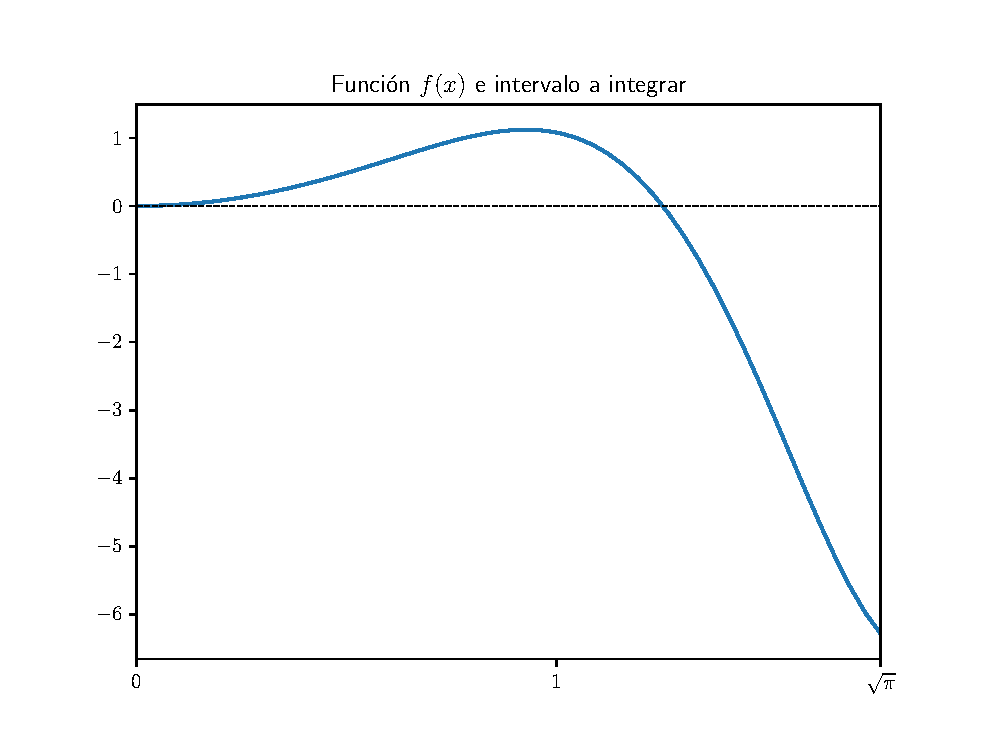
\includegraphics[scale=0.55]{Imagenes/integracion_ejercicio_Romberg_01.eps}
\end{figure}
\end{frame}
\begin{frame}
\frametitle{Camino 1}
Aquí tendrían que utilizar su propuesta de código para la regla recursiva del trapecio y luego la integración de Romberg.
\\
\bigskip
\pause
Sería el camino \enquote{manual} para la solución.
\end{frame}
\begin{frame}[allowframebreaks, plain, fragile]
\frametitle{Camino 1}
\begin{lstlisting}[caption=Función para la regla recursiva del trapecio]
def trapecio_recursiva(f, a, b, Iviejo, k):
    pass
    # aqui va el codigo que hay que desarrollar
\end{lstlisting}
\end{frame}
\begin{frame}[allowframebreaks, plain, fragile]
\begin{lstlisting}[caption=Función para la integración de Romberg]
def romberg(f, a, b, tol=1.0e-6):
    pass
    # aqui va el otro codigo que hay que desarrollar
\end{lstlisting}
\end{frame}
\begin{frame}[allowframebreaks, fragile]
\frametitle{Propuesta de código para resolver el ejercicio}
\begin{lstlisting}[caption=Código que evalúa la integral con el método de Romberg]
from moduloDiferencias import trapecio_recursiva
from moduloIntegracion import romberg
import numpy as np

def f(x): return 2.0*(x**2) * np.cos(x**2)

I, n = romberg(f, 0, np.sqrt(np.pi))

print('\nIntegral = {0:1.6f}'.format(I))
print('\nPaneles = {0:}'.format(n))
\end{lstlisting}
\end{frame}
\begin{frame}[fragile]
\frametitle{Resultado}
Luego de ejecutar el código, tendremos el siguiente resultado:
\pause
\begin{verbatim}
Integral = -0.894831

Paneles = 64
\end{verbatim}
\pause
Este resultado es más eficiente que calculado solo con la regla recursiva del trapecio, \pause resolviendo la integral con éste método, se requieren de $4096$ paneles.
\end{frame}

\subsection{La función \texttt{integrate.romberg}}

\begin{frame}
\frametitle{Usando la función \texttt{romberg} de \texttt{scipy}}
En la presentación anterior ya hemos presentado el uso de la función \funcionazul{scipy.integrate.quad} para integrar una función.
\\
\medskip
\pause
De la misma librería, tomamos la función \funcionazul{scipy.integrate.romberg}, que realiza una integración con la técnica de Romberg.
\end{frame}
\begin{frame}[fragile]
\frametitle{\texttt{scipy.integrate.romberg}}
Los parámetros mínimos para esta función son:
\\
\bigskip
\pause
\funcionazul{romberg(f, a, b, show=False)}
\\
\bigskip
\pause
Donde:
\setbeamercolor{item projected}{bg=blue,fg=yellow}
\setbeamertemplate{enumerate items}{%
\usebeamercolor[bg]{item projected}%
\raisebox{1.5pt}{\colorbox{bg}{\color{fg}\footnotesize\insertenumlabel}}%
}
\begin{enumerate}[<+->]
\item $f$ es la función a integrar.
\item $a$ es el límite inferior de integración.
\item $b$ es el límite superior de integración.
\end{enumerate}
\end{frame}
\begin{frame}[fragile]
\frametitle{Lo que devuelve \texttt{integrate.romberg}}
Esta función devuelve la integral de una función (función de una variable) en el intervalo $[a, b]$.
\\
\medskip
\pause
Si \funcionazul{show=1}, se muestra el arreglo triangular de resultados intermedios.
\end{frame}
\begin{frame}[fragile]
\frametitle{Código con scipy}
\begin{lstlisting}[caption=Integración de Romberg con scipy]
from numpy import cos, sqrt, pi
from scipy.integrate import romberg

def f(x): return 2.0 * (x**2) * cos(x**2)

resultado = romberg(f, 0, sqrt(pi), show=True)

print(resultado)
\end{lstlisting}
\end{frame}
\begin{frame}
\frametitle{Tabla de resultados}
\fontsize{6}{6}\selectfont
\setlength\arraycolsep{2pt}
\begin{tabular}{c c c c c c c c }
 Steps	&	StepSize	&	Results	 \\ \hline							
     $1$	&	$1.772454$	&	$-5.568328$ \\ \hline 
     $2$	&	$0.886227$	&	$-1.799813$	&	$-0.543642$ \\ \hline
     $4$	&	$0.443113$	&	$-1.034769$	&	$-0.779755$	&	\ldots \\ \hline
     $8$	&	$0.221557$	&	$-0.925214$	&	$-0.888695$	&	\ldots	&	\\ \hline
    $16$	&	$0.110778$	&	$-0.902166$	&	$-0.894484$	&	\ldots	&	\\ \hline
    $32$	&	$0.055389$	&	$-0.896649$	&	$-0.894810$	&	\ldots	&	$-0.894831$ \\ \hline
    $64$	&	$0.027695$	&	$-0.895285$	&	$-0.894830$	&	\ldots	&	$-0.894831$	&	$-0.894831$ \\ \hline
   $128$	&	$0.013847$	&	$-0.894945$	&	$-0.894831$	&	\ldots	&	$-0.894831$	&	$-0.894831$	&	$-0.894831$ 
\end{tabular}
\\
\bigskip
\fontsize{12}{12}\selectfont
The final result is $-0.894831469484$ after $129$ function evaluations.
\end{frame}
% \begin{frame}
% \frametitle{Ejercicio de clase}
% Evalúa la siguiente integral con el procedimiento de Romberg:
% \[ \scaleint{6ex}_{\bs 0}^{\frac{\pi}{4}} \dfrac{\dd{x}}{\sqrt{\sin x}} \]
% \end{frame}
% \begin{frame}
% \frametitle{Ejercicio de clase}
% Vemos que la integral es impropia, por lo que hay que manejarla de tal manera que se remueva la singularidad, en este caso, mediante un cambio de variable, para luego usar \funcionazul{scipy.integrate.romberg} con los respectivos límites de integración.
% \end{frame}
% \begin{frame}
% \frametitle{Ejercicio}
% Evalúa la integral
% \[ \scaleint{6ex}_{\bs 0}^{2} (x^{5} + 3 \: x^{3} - 2) \dd{x}\]
% por el método de integración de Romberg.
% \end{frame}

\section{Cuadraturas Gaussianas}
\frame{\tableofcontents[currentsection, hideothersubsections]}
\subsection{Definiciones}

\begin{frame}
\frametitle{Cuadraturas Gaussianas}
Hemos visto que las fórmulas de Newton-Cotes funcionan muy bien para aproximar la intregral:
\pause
\begin{align*}
\scaleint{6ex}_{\bs a}^{b} f (x) \dd{x}
\end{align*}
si $f (x)$ es una función suave, como los polinomios.
\end{frame}
\begin{frame}
\frametitle{Cuadraturas Gaussianas}
La aproximación también aplica para las cuadraturas Gaussianas, ya que son buenas para estimar integrales de la forma:
\pause
\begin{align*}
\scaleint{6ex}_{\bs a}^{b} w(x) f(x) \dd{x}
\end{align*}
donde $w (x)$ se denomina \textcolor{cerise}{función de peso o ponderación}, éstas pueden contener \textocolor{red}{singularidades}, siempre y cuando sean integrables.
\end{frame}
\begin{frame}
\frametitle{Cuadraturas Gaussianas}
Un ejemplo de este tipo, es la integral:
\pause
\begin{align*}
\scaleint{6ex}_{\bs 0}^{1} \left( 1 + x^{2} \right) \:  \ln(x) \: \dd{x}
\end{align*}
\\
\bigskip
\pause
En el caso de que algún (o ambos) límite(s) de integración sean infinitos:
\pause
\begin{align*}
\scaleint{6ex}_{\bs 0}^{\infty} \exp(-x) \: \sin x \: \dd{x}
\end{align*}
éstos se pueden reacomodar para calcular la integral.
\end{frame}
\begin{frame}
\frametitle{Fórmulas de integración Gaussianas}
Las fórmulas de integración Gaussianas tiene la misma forma de las reglas de Newton-Cotes:
\pause
\begin{align*}
I = \nsum_{i=0}^{n} A_{i} \, f (x_{i})
\end{align*}
donde $I$ representa la aproximación al valor de la integral, \pause la diferencia radica en la forma en que se determinan los pesos $A_{i}$ y abscisas nodales $x_{i}$.
\end{frame}
\begin{frame}
\frametitle{Fórmulas de integración Gaussianas}
En la integración de Newton-Cotes los nodos se distribuyen uniformemente en $(a, b)$, es decir, estaban ya predeterminadas sus ubicaciones.
\end{frame}
\begin{frame}
\frametitle{Fórmulas de integración Gaussianas}
En la cuadratura de Gauss, se eligen los nodos y los pesos de modo que la ecuación para $I$ es la integral exacta si $f (x)$ es un polinomio de grado $2 \, n + 1$ o menor, es decir:
\pause
\begin{align*}
\scaleint{6ex}_{\bs a}^{b} w(x) \, P_{m} (x) \dd{x} = \nsum_{i=0}^{n} A_{i} \, P_{m} (x_{i}), \hspace{1cm} m \leq 2 \, n + 1
\end{align*}
\end{frame}
\begin{frame}
\frametitle{Fórmulas de integración Gaussianas}
Una manera de determinar los pesos y las abscisas es sustituir:
\pause
\begin{align*}
P_{0} (x) &= 1 \\
P_{1} (x) &= x, \\
&\ldots  \\
P_{2 \: n + 1} (x) &= x^{2 \: n + 1}
\end{align*}
en la ecuación anterior.
\end{frame}
\begin{frame}
\frametitle{Expresión para la cuadratura}
Para luego resolver el sistema de $2 \: n + 2$ ecuaciones:
\pause
\begin{align*}
\scaleint{6ex}_{\bs a}^{b} \: w(x) \: x^{j} \: \dd{x} = \nsum_{i = 0}^{n} \: A_{i} \: x_{i}^{j}, \hspace{1cm} j = 0, 1, \ldots, 2 \: n + 1 \end{align*}
para las incógnitas $A_{i}$ y $x_{i}$.
\end{frame}
\begin{frame}
\frametitle{Ejemplo con una función $w (x)$}
Sea la función de peso:
\pause
\begin{align*}
w (x) = \exp(-x)
\end{align*}
y con $a = 0$, $b = \infty$ y $n =  1$.
\\
\bigskip
\pause
Las cuatro ecuaciones ($j= 0, 1, 2, 3$) que determinan $x_{0}$, $x_{1}$, $A_{0}$ y $A_{1}$ son:
\end{frame}
\begin{frame}
\frametitle{Ejemplo con una función $w (x)$}
\begin{eqnarray*}
\begin{aligned}
\scaleint{6ex}_{\bs 0}^{\infty} \exp(-x) \dd{x} &= A_{0} + A_{1} \\ \pause
\scaleint{6ex}_{\bs 0}^{\infty} \exp(-x) \, x \dd{x} &= A_{0} \, x_{0} + A_{1} \, x_{1} \\ \pause
\scaleint{6ex}_{\bs 0}^{\infty} \exp(-x) \, x^{2} \dd{x} &= A_{0} \, x_{0}^{2}+ A_{1} \, x_{1}^{2} \\ \pause
\scaleint{6ex}_{\bs 0}^{\infty} \exp(-x) \, x^{3} \dd{x} &= A_{0} \, x_{0}^{3} + A_{1} \, x_{1}^{3} \\
\end{aligned}
\end{eqnarray*}
\end{frame}
\begin{frame}
\frametitle{Evaluando las integrales}
Evaluando las integrales, obtenemos:
\pause
\begin{eqnarray*}
\begin{aligned}
A_{0} + A_{1} &= 1 \\ \pause
A_{0} \, x_{0} + A_{1} \, x_{1} &= 1 \\ \pause
A_{0} \, x_{0}^{2} + A_{1} \, x_{1}^{2} &= 2 \\ \pause
A_{0} \, x_{0}^{3} + A_{1} \, x_{1}^{3} &= 6
\end{aligned}
\end{eqnarray*}
\end{frame}
\begin{frame}
\frametitle{Solución del sistema}
Cuya solución es:
\pause
\begin{eqnarray*}
\begin{aligned}
x_{0} &= 2 - \sqrt{2} \pause \hspace{0.75cm} A_{0} = \dfrac{\sqrt{2} + 1}{2\sqrt{2}} \\[0.5em] \pause
x_{1} &= 2 + \sqrt{2} \pause \hspace{0.75cm} A_{1} = \dfrac{\sqrt{2} - 1}{2\sqrt{2}}
\end{aligned}
\end{eqnarray*}
\end{frame}
\begin{frame}
\frametitle{Resultado de la integración}
Por tanto la fórmula de integración obtenida es:
\pause
\begin{eqnarray*}
\begin{aligned}
&\scaleint{6ex}_{\bs 0}^{\infty} \exp(-x) \, f (x) \dd{x} \simeq \\[0.5em]
& \simeq \dfrac{1}{2 \, \sqrt{2}} \big[ \big( \sqrt{2} + 1 \big) \, f \,  \big( 2 - \sqrt{2} \big) + \big( \sqrt{2} - 1 \big) f \big( 2  + \sqrt{2} \big) \big]
\end{aligned}
\end{eqnarray*}
\pause
Debido a la no linealidad de las ecuaciones, este enfoque no va a funcionar bien para valores grandes de $n$.
\end{frame}
\begin{frame}
\frametitle{Calculando nodos y pesos}
Hay métodos prácticos para calcular $x_{i}$ y $A_{i}$ que requieren un cierto conocimiento de los polinomios ortogonales y su relación con la cuadratura de Gauss.
\\
\bigskip
\pause
Hay, sin embargo, varias fórmulas \enquote{clásicas} de integración Gaussianas para los cuales, las abscisas y pesos han sido calculados y tabulados con gran precisión.
\end{frame}
\begin{frame}
\frametitle{Calculando nodos y pesos}
Estas fórmulas se pueden utilizar sin conocer la teoría detrás de ellas, ya que todo lo que uno necesita para la integración de Gauss son los valores de $x_{i}$ y $A_{i}$.
\end{frame}

\subsection{Polinomios ortogonales}

\begin{frame}
\frametitle{Polinomios ortogonales}
Los \textocolor{blue-violet}{polinomios ortogonales} se utilizan en muchas áreas de la física, de la matemática y del análisis numérico; se han estudiado a fondo y muchas de sus propiedades ya son conocidas. 
\end{frame}
\begin{frame}
\frametitle{Polinomios ortogonales}
Los polinomios $\varphi_{n}(x)$, con $n = 0, 1, 2,\ldots$ ($n$ es el grado del polinomio) se dice que forman un conjunto ortogonal en el intervalo $(a, b)$ con respecto a la función de peso $w(x)$ si:
\pause
\begin{align*}
\scaleint{6ex}_{\bs a}^{b} w (x) \, \varphi_{m} (x) \, \varphi_{n} (x) \dd{x} = 0, \hspace{0.5cm} m \neq n
\end{align*}
\end{frame}
\begin{frame}
\frametitle{Polinomios ortogonales}
El conjunto se determina (con excepción de un factor constante) por: la elección de la función de peso y los límites de integración.
\\
\bigskip
\pause
Es decir, cada conjunto de polinomios ortogonales se asocia con ciertos $w(x)$, $a$ y $b$. \pause El factor constante se especifica de manera estandarizada.
\end{frame}
\begin{frame}
\frametitle{Polinomios ortogonales más utilizados}
A continuación se enlistan algunos de los polinomios ortogonales clásicos, la última columna indica la estandarización usada.
\end{frame}
\begin{frame}
\frametitle{Polinomios ortogonales}
Legendre: $P_{n} (x)$  \hspace{0.5cm} $a = -1$, $b = 1$, $w (x) = 1$ \\[0.5em]
$\scaleint{6ex}_{\bs -1}^{1} \left[ \varphi_{n} (x)\right]^{2} \dd{x} = \dfrac{2}{2 \, n + 1}$
\\[0.5em]
\rule{10cm}{1pt}
\\[0.5em]
\pause
Chebyshev: $T_{n} (x)$ \hspace{0.5cm} $a = -1$, $b = 1$, $w (x) = (1 - x^{2})^{-1/2}$ \\[0.5em]
$\scaleint{6ex}_{\bs -1}^{1} (1 - x^{2})^{-1/2} \left[ \varphi_{n} (x)\right]^{2} \dd{x} = \dfrac{\pi}{2} \hspace{0.2cm} (n > 0)$
\end{frame}
\begin{frame}
\frametitle{Polinomios de Legendre}
\begin{figure}
  \centering
  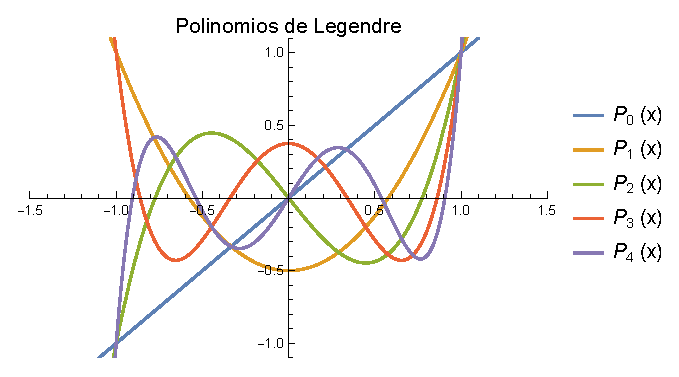
\includegraphics[scale=0.9]{Imagenes/plot_Legendre_01.eps}
\end{figure}
\end{frame}
\begin{frame}
\frametitle{Polinomios de Chebyshev}
\begin{figure}
  \centering
  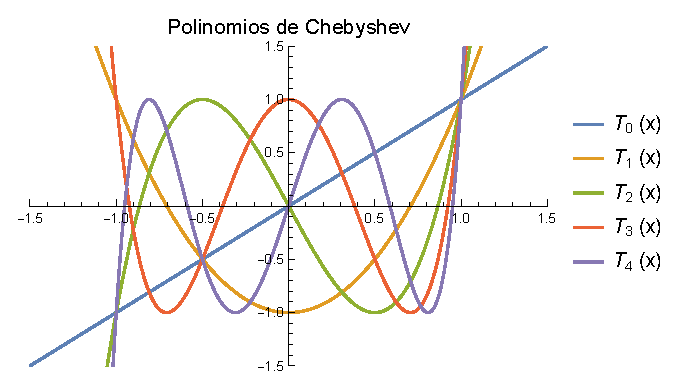
\includegraphics[scale=0.9]{Imagenes/plot_Chebyshev_01.eps}
\end{figure}
\end{frame}
\begin{frame}
\frametitle{Polinomios ortogonales}
Laguerre: $L_{n} (x)$ \hspace{0.5cm} $a = 0$, $b = \infty$, $w (x) = e^{-x}$ \\[0.5em]
$\scaleint{6ex}_{\bs 0}^{\infty} e^{-x} \, \left[ \varphi_{n} (x)\right]^{2} \dd{x} = 1$ 
\\[0.5em]
\rule{10cm}{1pt}
\\[0.5em]
\pause
Hermite: $H_{n} (x)$ \hspace{0.5cm} $a = -\infty$, $b = \infty$, $w (x) = e^{x^{2}}$ \\
$\scaleint{6ex}_{\bs -\infty}^{\infty} e^{x^{2}} \, \left[ \varphi_{n} (x) \right]^{2} \dd{x} = \sqrt{\pi} \, 2^{n} \, n!$
\end{frame}
\begin{frame}
\frametitle{Polinomios de Laguerre}
\begin{figure}
  \centering
  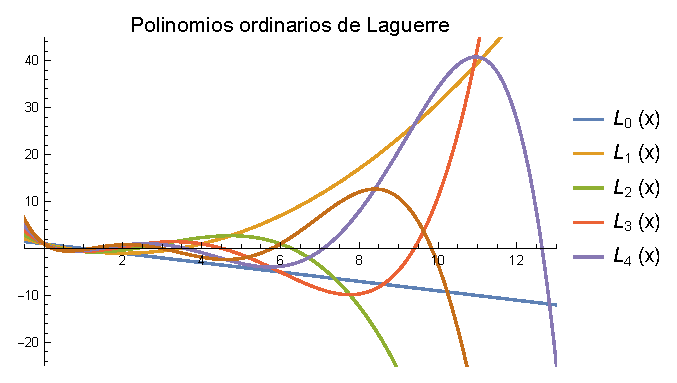
\includegraphics[scale=0.9]{Imagenes/plot_Laguerre_01.eps}
\end{figure}
\end{frame}
\begin{frame}
\frametitle{Polinomios de Hermite}
\begin{figure}
  \centering
  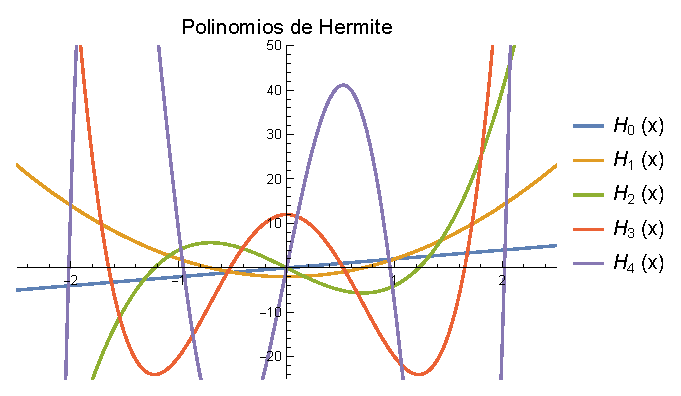
\includegraphics[scale=0.9]{Imagenes/plot_Hermite_01.eps}
\end{figure}
\end{frame}
\begin{frame}
\frametitle{Relaciones de recurrencia}
Los polinomios ortogonales cumplen relaciones de recurrencia de la forma:
\begin{align*}
a_{n} \varphi_{n+1} (x) = (b_{n} + c_{n} x) \varphi_{n} (x) - d_{n} \varphi_{n-1} (x) 
\end{align*}
Si los dos primeros polinomios del conjunto se conocen, los otros elementos del conjunto pueden calcularse de la ecuación anterior. 
\end{frame}
\begin{frame}
\frametitle{Coeficientes de las reglas de recurrencia}
Los coeficientes en la fórmula de recurrencia, junto con $\varphi_{0} (x)$ y $\varphi_{1} (x)$ son:
\pause
\begin{table}
\centering
\fontsize{12}{12}\selectfont
\begin{tabular}{| l | c | c | c | c | c | c |}
\hline
Nombre & $\varphi_{0}(x)$ & $\varphi_{1}(x)$ & $a_{n}$ & $b_{n}$ & $c_{n}$ & $d_{n}$ \\ \hline
Legendre & $1$ & $x$ & $n+1$ & $0$ & $2n+1$ & n \\
Chebyshev & $1$ & $x$ & $1$ & $0$ & $2$ & $1$ \\
Laguerre & $1$ & $1-x$ & $n+1$ & $2n+1$ & $-1$ & $n$ \\
Hermite & $1$ & $2x$ & $1$ & $0$ & $2$ & $2$ \\ \hline
\end{tabular}
\end{table}
\end{frame}
\begin{frame}
\frametitle{Otra manera para obtener los polinomios}
Los polinomios ortogonales clásicos también se pueden obtener de las fórmulas:
\pause
\begin{align*}
P_{n} (x) &= \dfrac{(-1)^{n}}{2^{n}n!} \dv[n]{x} \left[ \left( 1 - x^{2} \right)^{n} \right] \\[1em]
T_{n} (x) &= \cos(n \, \cos^{-1} x), \hspace{0.3cm} n > 0 \\[1em]
L_{n} (x) &= \dfrac{e^{x}}{n!} \dv[n]{x} \left( x^{n} \, e^{-x} \right) \\[1em]
H_{n} (x) &= (-1)^{n} e^{x^{2}} \dv[n]{x} \left(e^{x^{2}} \right)
\end{align*}
\end{frame}
\begin{frame}
\frametitle{Derivadas de los polinomios ortogonales}
Las derivadas de los polinomios anteriores se pueden calcular de:
\pause
\begin{align*}
(1 - x^{2}) \: \pderivada{P}_{n} (x) &= n \: [ -x \: P_{n} (x) + P_{n - 1} (x) ] \\[1em]
(1 - x^{2}) \: \pderivada{T}_{n} (x) &= n \: [-x \: T_{n} (x) + n \: p \: T{n - 1} (x) ] \\[1em]
x \: \pderivada{L}_{n} \: (x) &= n \: [ L_{n} (x) - L_{n - 1} (x) ] \\[1em]
\pderivada{H}_{n} (x) &= 2 \: n \:  H_{n - 1} (x)
\end{align*}
\end{frame}
\begin{frame}
\frametitle{Propiedades de los polinomios}
Algunas propiedades los polinomios ortogonales que son relevantes para la preceso de integración Gaussiana son:
\pause
\setbeamercolor{item projected}{bg=black,fg=white}
\setbeamertemplate{enumerate items}{%
\usebeamercolor[bg]{item projected}%
\raisebox{1.5pt}{\colorbox{bg}{\color{fg}\footnotesize\insertenumlabel}}%
}
\begin{enumerate}[<+->]
\item $\varphi_{n} (x)$ tiene $n$ distintos ceros en el intervalo $(a,b)$.
\item Los ceros de $\varphi_{n} (x)$ están entre los ceros de $\varphi_{n + 1} (x)$.
\item Cualquier polinomio $P_{n} (x)$ de grado $n$ puede expresarse de la forma:
\begin{align*}
P_{n} (x) = \nsum_{i=0}^{n} c_{i} \: \varphi_{i} (x)
\end{align*}
\seti
\end{enumerate}
\end{frame}
\begin{frame}
\frametitle{Propiedades de los polinomios}
\setbeamercolor{item projected}{bg=black,fg=white}
\setbeamertemplate{enumerate items}{%
\usebeamercolor[bg]{item projected}%
\raisebox{1.5pt}{\colorbox{bg}{\color{fg}\footnotesize\insertenumlabel}}%
}
\begin{enumerate}
\conti
\item Se deduce de la ecuación anterior y de la propiedad de ortogonalidad que:
\begin{align*}
\scaleint{6ex}_{\bs a}^{b} w (x) \, P_{n} (x) \, \varphi_{n+m} (x) \dd{x} = 0, \hspace{0.4cm} m \geq 0
\end{align*}
\end{enumerate}
Nota: Si hablamos del polinomio $P_{n} (x)$ no hay que confundirlo con la función especial de Legendre $P_{n} (x)$, ya que se ocupa la misma letra. 
\end{frame}

\subsection{Abscisas nodales y los pesos}

\begin{frame}
\frametitle{Deduciendo las abscisas nodales y los pesos}
Hay dos teoremas importantes que son de gran utilidad para apoyarnos y tomar sus resultados para la integración Gaussiana, la demostración es relativamente sencilla, pero no los demostraremos aquí, puede ser un buen ejercicio fuera de clase.
\end{frame}
\begin{frame}
\frametitle{Teorema 1}
\begin{miteorema}
Las abscisas nodales $x_{0}, x_{1}, \ldots, x_{n}$ son los ceros del polinomio $\varphi_{n+1} (x)$  que pertenece al conjunto ortogonal definido por:
\begin{align*}
\scaleint{6ex}_{\bs a}^{b} w (x) \: \varphi_{m} (x) \: \varphi_{n} (x) \: \dd{x} = 0, \hspace{0.5cm} m \neq n
\end{align*}
\end{miteorema}
\end{frame}
\begin{frame}
\frametitle{Teorema 2}
\begin{miteorema}
\begin{align*}
A_{i} = \scaleint{6ex}_{\bs a}^{b} w (x) \: \mathcal{L}_{i} (x) \: \dd{x}, \hspace{1cm} i = 0, 1, \ldots, n
\end{align*}
donde $\mathcal{L}_{i} (x)$ son las funciones cardinales de Lagrange que abarcan los nodos $x_{0}, x_{1}, \ldots, x_{n}$.
\end{miteorema}
\end{frame}
\begin{frame}
\frametitle{Cálculo de las raíces}
No es difícil calcular los ceros $x_{i}$, $i = 0, 1, \ldots, n$ de un polinomio $\varphi_{n + 1} (x)$ que pertenece a un conjunto ortogonal, podemos usar alguno de los métodos discutidos en la parte de cálculo de raíces.
\\
\bigskip
\pause
Una vez conocidos los ceros, los pesos $A_{i}$, $i = 0, 1, \ldots, n$ pueden calcularse de la ecuación anterior.
\end{frame}
\begin{frame}
\frametitle{Fórmulas para calcular los pesos}
Se puede demostrar que los pesos se pueden calcular a partir de:
\pause
\begin{align*}
\text{Gauss-Legendre   }  A_{i} &= \dfrac{2}{(1 - x^{2}_{i}) \: \left[\pderivada{P}_{n + 1} (x_{i}) \right]^{2}} \\[1em]
\text{Gauss-Laguerre   } A_{i} &= \dfrac{1}{x_{i} \: \left[\pderivada{L}_{n + 1} (x_{i}) \right]^{2}} \\[1em]
\text{Gauss-Hermite   } A_{i} &= \dfrac{2^{n + 2} \: (n + 1)! \: \sqrt{\pi}}{\left[ \pderivada{H}_{n + 1} (x_{i}) \right]^{2}}
\end{align*}
\end{frame}

\subsection{Error en la cuadratura Gaussiana}

\begin{frame}
\frametitle{Error en la cuadratura Gaussiana}
El error debido al truncamiento en este tipo de cuadratura es:
\pause
\begin{align*}
E = \scaleint{6ex}_{\bs a}^{b} w (x) \: f (x) \: \dd{x}  - \nsum_{i = 0}^{n} A_{i} \, f (x_{i})
\end{align*}
\pause
que es de la forma $E = K (n) \, f^{2 \: n + 2} (c) $, donde $a < c < b$, el valor de $c$ no se conoce, solamente los extremos.
\end{frame}
\begin{frame}
\frametitle{Error en la cuadratura Gaussiana}
La expresión para $K (n)$ depende de la cuadratura en particular que se esté utilizando.
\\
\bigskip
\pause
Si las derivadas de $f (x)$ se pueden evaluar, el error de las fórmulas es útil para estimar el error en el intervalo.
\end{frame}
\begin{frame}
\frametitle{Gauss-Legendre: abscisas y pesos}
Vamos a mencionar la expresión para algunas fórmulas de integración por cuadraturas gaussianas.
\\
\bigskip
\pause
La tabla de abscisas y pesos que se presenta a continuación, cubre para $n = 1$ a $5$, y se redondea a seis decimales.
\end{frame}
\begin{frame}
\frametitle{Gauss-Legendre: abscisas y pesos}
Las operaciones con estos valores, se considera que funcionan bien si se hacen las cuentas a mano, en caso de requerir una mayor precisión o incluir un número  mayor de nodos, será necesario usar la computadora.
\end{frame}
\begin{frame}[plain]
\frametitle{Cuadratura de Gauss-Legendre}
La aproximación para la cuadratura de Gauss-Legendre es:
\begin{align*}
\scaleint{6ex}_{\bs -1}^{1} f(\xi) \: \dd{\xi} \approx \nsum_{i = 0}^{n} A_{i} \: f (\xi_{i})
\end{align*}
\end{frame}
\begin{frame}
\frametitle{Gauss-Legendre: abscisas y pesos}
\fontsize{10}{10}\selectfont
\begin{center}
\begin{tabular}{|c c c | c c c|}
\hline
$\pm \xi_{i}$ &       & $A_{i}$    & $\pm \xi_{i}$ &       & $A_{i}$ \\ \hline
             & $n = 1$ &            &               & $n = 4$ &         \\ %\hline
$0.577350$    &       & $1.000000$ & $0.000000$    &       & $0.568889$ \\ %\hline
             & $n = 2$ &            & $0.538469$    &       & $0.478629$ \\ %\hline
$0.000000$    &       & $0.888889$ & $0.906180$    &       & $0.236927$ \\ %\hline
$0.774597$    &       & $0.555556$ &               & $n = 5$ &            \\ %\hline
             & $n = 3$ &            & $0.238619$    &       & $0.467914$ \\ %\hline
$0.339981$    &       & $0.652145$ & $0.661209$    &       & $0.360762$ \\ %\hline
$0.861136$    &       & $0.347855$ & $0.932470$    &       & $0.171324$ \\ \hline
\end{tabular}
\end{center}
\end{frame}
\begin{frame}
\frametitle{Cuadratura de Gauss-Legendre}
La cuadratura de Gauss-Legendre es la más utilizada. 
\\
\bigskip
\pause
Nótese que los nodos están colocados simétricamente sobre $\xi = 0$, y los pesos asociados al par de nodos simétricos, son iguales, \pause i.e. para $n = 1$, tenemos que $\xi_{0} = - \xi_{1}$ y $A_{0} = A_{1}$.
\end{frame}
\begin{frame}
\frametitle{Error en la cuadratura}
El error de truncamiento está dado por:
\pause
\begin{align*}
E = \dfrac{2^{2n+3} \, [(n + 1)!]^{4}}{(2 \, n + 3)[(2 \, n + 2)!]^{3}} \, f^{(2n+2)} (c), \hspace{1cm} -1 < c < 1
\end{align*}
\end{frame}
\begin{frame}
\frametitle{Mapeo en el intervalo}
Para usar la cuadratura de Gauss-Legendre en la integral:
\pause
\begin{align*}
\scaleint{6ex}_{\bs a}^{b} \: f (x) \dd{x}
\end{align*}
primero hay que \enquote{mapear} el intervalo de integración $(a,b)$ al intervalo \enquote{estándar} $(-1, 1)$, \pause para ello, usamos la transformación:
\pause
\begin{align*}
x = \dfrac{b + a}{2} + \dfrac{b - a}{2} \xi
\end{align*}
\end{frame}
\begin{frame}
\frametitle{Nueva expresión de la cuadratura}
Ahora $\dd{x} = d \xi (b-a)/2$, y la cuadratura toma la expresión:
\pause
\begin{align*}
\scaleint{6ex}_{\bs a}^{b} f (x) \dd{x} \approx \dfrac{b - a}{2} \nsum_{i=0}^{n} A_{i} \, f (x_{i})
\end{align*}
\end{frame}
\begin{frame}
\frametitle{Estimación del error}
El error por truncamiento, se expresa como:
\pause
\begin{align*}
E = \dfrac{(b - a)^{2n+3} [(n + 1)!]^{4}}{(2 \, n + 3)[(2 \ n + 2)!]^{3}} f^{(2n+2)} (c), \hspace{0.7cm} a < c < b
\end{align*}
\end{frame}
% % \begin{frame}<
% % \frametitle{Ej<ercicio para el examen}
% % Te pedimos que entregues una lista con los pesos y nodos para las siguientes cuadraturas:
% % \begin{enumerate}
% % \item Gauss-Chebyshev
% % \[\scaleint{6ex}_{\bs 1}^{1} (1-x^{2})^{-1/2} f(x) \approx \dfrac{\pi}{n+1} \sum_{i=0}^{n} f(x_{i}) \]
% % \item Gauss-Laguerre
% % \[  \scaleint{6ex}_{\bs 0}^{\infty} e^{-x} f(x) \dd{x} \approx \sum_{i=0}^{n} A_{i} f(x_{i}) \]
% % \end{enumerate}
% % \end{frame}
% % \begin{frame}
% % \frametitle{Ejercicio para el examen}
% % \begin{enumerate}
% % \item Gauss-Hermite
% % \[ \scaleint{6ex}_{\bs -\infty}^{\infty} e^{-x^{2}} f(x) \dd{x} \approx \sum_{i=0}^{n} A_{i} f(x_{i}) \]
% % \end{enumerate}
% % \end{frame}
% \begin{frame}
% \frametitle{¿Aquí termina todo respecto a la integración numérica?}
% Como sabemos de los cursos de cálculo, podemos considerar ahora un proceso de integración para calcular integrales de funciones con dos y hasta tres variables, recurriendo a las técnicas mostradas.
% \\
% \medskip
% ¿Cómo construimos un algoritmo para ello?
% \\
% \medskip
% El proceso no es complicado pero requiere una revisión cuidadosa, con \python{} podemos hacer el proceso más sencillo para calcular una integral doble o triple, pero no está demás que te las ingenies para desarrollar un código!!
% \end{frame}
\begin{frame}
\frametitle{Ejercicio cuadratura Gaussiana}
Evaluar la integral:
\begin{align*}
\scaleint{6ex}_{\bs -1}^{1} (1 - x^{2})^{3/2} \; \dd{x}
\end{align*}
con la mayor precisión posible, usando una cuadratura Gaussiana.
\end{frame}
\begin{frame}
\frametitle{Modo clásico}
El modo normal de resolver mediante una cuadratura Gaussiana, es calcuar los nodos para una cuadratura de tipo Gauss-Legendre.
\\
\bigskip
\pause
Por lo que tendríamos que ocupar las expresiones que nos devuelvan los ceros de los polinomios. 
\end{frame}

\subsection{Funciones \texttt{quadrature}}

\begin{frame}[fragile]
\frametitle{Usando \texttt{scipy.integrate.quadrature}}
Para usar la función \funcionazul{scipy.integrate.cuadrature}, hay que considerar la sintaxis mínima:
\pause
\\
\bigskip
\funcionazul{scipy.integrate.quadrature(func, a, b, tol=1.49e-08, maxiter=50)}
\\
\bigskip
\pause
Esta función calcula la integral definida usando una cuadratura gaussina con tolerancia fija.
\end{frame}
\begin{frame}
\frametitle{Argumentos de \texttt{quadrature}}
Los argumentos son:
\setbeamercolor{item projected}{bg=red,fg=white}
\setbeamertemplate{enumerate items}{%
\usebeamercolor[bg]{item projected}%
\raisebox{1.5pt}{\colorbox{bg}{\color{fg}\footnotesize\insertenumlabel}}%
}
\begin{enumerate}[<+->]
\item \funcionazul{func} : una función, ya sea una función de \python{} o una expresión.
\item \funcionazul{a} : dato de tipo \texttt{float}, que representa el límite inferior de integración.
\item \funcionazul{b} : dato de tipo \texttt{float}, que representa el límite superior de integración.
\seti
\end{enumerate}
\end{frame}
\begin{frame}
\frametitle{Argumentos de \texttt{quadrature}}
\setbeamercolor{item projected}{bg=red,fg=white}
\setbeamertemplate{enumerate items}{%
\usebeamercolor[bg]{item projected}%
\raisebox{1.5pt}{\colorbox{bg}{\color{fg}\footnotesize\insertenumlabel}}%
}
\begin{enumerate}
\conti    
\item \funcionazul{maxiter} : dato de tipo \texttt{int}, este argumento es opcional, representa el orden máximo para la quadratura Gaussiana.
\end{enumerate}
\end{frame}
\begin{frame}
\frametitle{Valores que devuelve la función}
La función devuelve:
\pause
\setbeamercolor{item projected}{bg=lilac,fg=white}
\setbeamertemplate{enumerate items}{%
\usebeamercolor[bg]{item projected}%
\raisebox{1.5pt}{\colorbox{bg}{\color{fg}\footnotesize\insertenumlabel}}%
}
\begin{enumerate}[<+->]
\item \funcionazul{val} : dato de tipo \texttt{float}, que representa la aproximación a la integral.
\item \funcionazul{err} : dato de tipo \texttt{float}, que representa el error en las últimas dos estimaciones de la integral.
\end{enumerate}
\end{frame}
\begin{frame}[fragile]
\frametitle{Código para el ejercicio}
\begin{lstlisting}[caption=Código para cuadratura Gaussiana]
from scipy.integrate import quadrature

def g(x): return (1 - x**2)**(3/2)

print(quadrature(g, -1., 1)[0])
\end{lstlisting}
\end{frame}
\begin{frame}
\frametitle{Solución al ejercicio}
El valor de la integral es $I = 1.17809716$
\begin{figure}
  \centering
  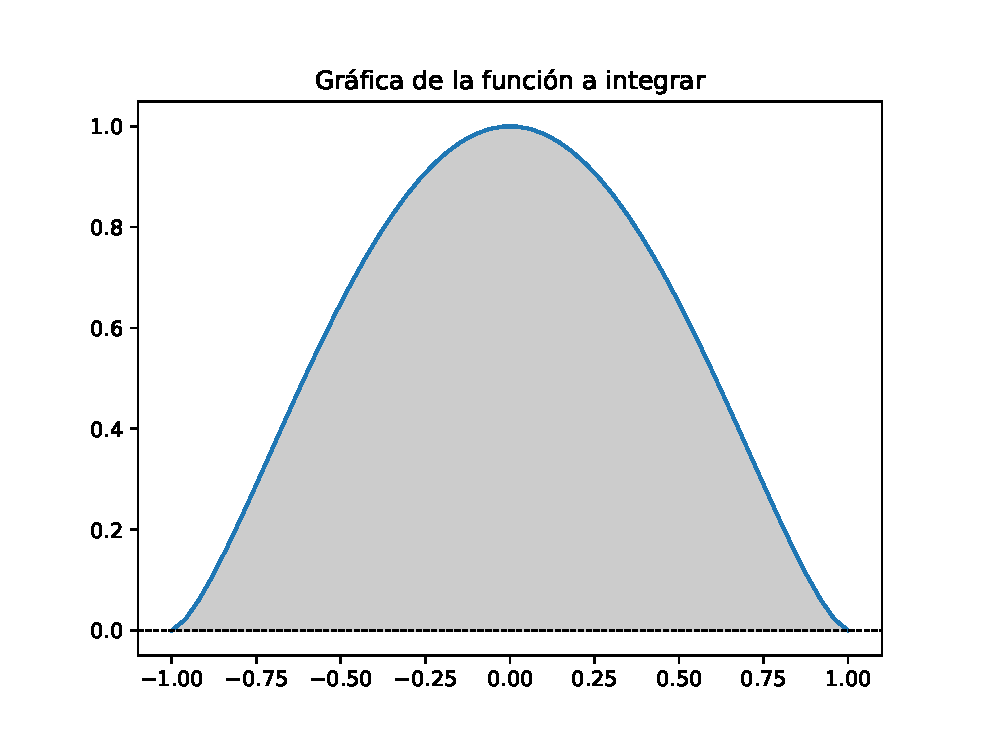
\includegraphics[scale=0.5]{Imagenes/cuadratura_01.eps}
\end{figure}
\end{frame}
\end{document}